\documentclass[12pt, fullpage,letterpaper]{article}

\usepackage[margin=1in]{geometry}
\usepackage{url}
\usepackage{amsmath}
\usepackage{amssymb}
\usepackage{xspace}
\usepackage{graphicx}
\usepackage{hyperref}
\usepackage{listings}

\newcommand{\semester}{Spring 2020}
\newcommand{\assignmentId}{1}
\newcommand{\releaseDate}{21 January, 2020}
\newcommand{\dueDate}{11:59pm, 8 Feb, 2020}

\newcommand{\bx}{{\bf x}}
\newcommand{\bw}{{\bf w}}

\title{CS 5350/6350: Machine Learining \semester}
\author{Torin McDonald, u0940253, Homework \assignmentId}
\date{Handed out: \releaseDate\\
	Due: \dueDate}


\title{CS 5350/6350: Machine Learining \semester}
\author{Homework \assignmentId}
\date{Handed out: \releaseDate\\
  Due date: \dueDate}

\begin{document}
\maketitle

\input{emacscomm}


\section{Decision Tree [40 points + 10 bonus]}

****NOTE: images of trees are in the appendix found at the end of the document

\begin{table}[h]
	\centering
	\begin{tabular}{cccc|c}
		$x_1$ & $x_2$ & $x_3$ & $x_4$ & $y$\\ 
		\hline\hline
		0 & 0 & 1 & 0 & 0 \\ \hline
		0 & 1 & 0 & 0 & 0 \\ \hline
		0 & 0 & 1 & 1 & 1 \\ \hline
		1 & 0 & 0 & 1 & 1 \\ \hline
		0 & 1 & 1 & 0.& 0\\ \hline
		1 & 1 & 0 & 0 & 0\\ \hline
		0 & 1 & 0 & 1 & 0\\ \hline
	\end{tabular}
	\caption{Training data for a Boolean classifier}
	%\caption{Training data for the alien invasion problem.}\label{tb-alien-train}
\end{table}

\begin{enumerate}
\item~[7 points] Decision tree construction. 
\begin{enumerate}
\item~[5 points] \\\\
For the first step, we find the best split for the data using information gain. 

We first find the current entropy for the set of examples, using the equation $H(p)=-\sum^k_{i=1}p_ilog(p_i)$

In this case, it is $-(2/7)*log2(2/7)-(5/7)*log2(5/7)=0.86312056856$

Now, we find the entropy for each feature, represented in this table. The entoropy is calculated using the same equation as above.

\begin{tabular}{|l|l|l|l|l|l|}
	\hline
	feature & p   & n   & tot & entropy       & Weighted \\ \hline
	x1(0)   & 1/5 & 4/5 & 5/7 & 0.72192809488 & 0.51566  \\ \hline
	x1 (1)  & 1/2 & 1/2 & 2/7 & 1             & 0.28571  \\ \hline
	x2(0)   & 2/3 & 1/3 & 3/7 & 0.91829583405 & 0.39356  \\ \hline
	x2(1)   & 0   & 1   & 4/7 & 0             & 0.00000  \\ \hline
	x3(0)   & 1/4 & 3/4 & 4/7 & 0.81127812445 & 0.00000  \\ \hline
	x3 (1)  & 1/3 & 2/3 & 3/7 & 0.91829583405 & 0.39356  \\ \hline
	x4 (0)  & 0   & 1   & 4/7 & 0             & 0.00000  \\ \hline
	x4 (1)  & 2/3 & 1/3 & 3/7 & 0.91829583405 & 0.39356  \\ \hline
	\end{tabular}

In the next step, we calculateed the expected entropy for each feature. This is done by multiplying the total fraction by the entropy for each value a specific feature can take, and then adding  them together foor each feature.

Finally, the information gain is calculated by subracting the expected entropy from the current entropy of the entire set of examples.


	\begin{tabular}{|l|l|l|}
	\hline
	feature & expected entropy & information gain \\ \hline
	x1      & 0.80138          & 0.06             \\ \hline
	x2      & 0.39356          & 0.47             \\ \hline
	x3      & 0.85714          & 0.01             \\ \hline
	x4      & 0.39356          & 0.47             \\ \hline
	\end{tabular}

Now, we pick x2 as the best attribute to split the data because it has the highest information gain (breaking the tie by first feature).

For each value of x2 (0 and 1), we add a new branch, and use the subset of examples S where the attribute= v:

Branch 1 (x2=0):

Sv=\begin{tabular}{|l|l|l|l|l|}
	\hline
	x1 & x2 & x3 & x4 & y \\ \hline
	0  & 0  & 1  & 0  & 0 \\ \hline
	0  & 0  & 1  & 1  & 1 \\ \hline
	1  & 0  & 0  & 1  & 1 \\ \hline
	\end{tabular}

Because Sv is not empty, we recursively call the id3 algorithm. 

We find the best split for this set of examples (logic is exactly the same as the first iteration explained above):

Current entropy = $-(1/3)*log2(1/3)-(2/3)*log2(2/3)=0.91829583405$

\begin{tabular}{|l|l|l|l|l|l|}
	\hline
	feature & p   & n   & tot & entropy & Weighted \\ \hline
	x1(0)   & 1/2 & 1/2 & 2/3 & 1       & 2/3      \\ \hline
	x1 (1)  & 1   & 0   & 1/3 & 0       & 0        \\ \hline
	x3(0)   & 1   & 0   & 1/3 & 0       & 0        \\ \hline
	x3 (1)  & 1/2 & 1/2 & 2/3 & 1       & 2/3      \\ \hline
	x4 (0)  & 0   & 1   & 1/3 & 0       & 0        \\ \hline
	x4 (1)  & 1   & 0   & 2/3 & 0       & 0        \\ \hline
	\end{tabular}


	\begin{tabular}{|l|l|l|}
		\hline
		feature & expected entropy & information gain \\ \hline
		x1      & 2/3              & 0.25162916738    \\ \hline
		x3      & 2/3              & 0.25162916738    \\ \hline
		x4      & 0                & 0.91829583405    \\ \hline
		\end{tabular}

The best attribute is x4,  loop through both values. Since neither subest is empty, we return the id3 algorithm again. In both the 0 and 1 cases, the subset will have the same label, so we return a leaf node with the label (0 for x4=0 and 1 for x4=1)

Branch 2 (x2=1):

Sv=\begin{tabular}{|l|l|l|l|l|}
	\hline
	x1 & x2 & x3 & x4 & y \\ \hline
	0  & 1  & 0  & 0  & 0 \\ \hline
	0  & 1  & 1  & 0. & 0 \\ \hline
	1  & 1  & 0  & 0  & 0 \\ \hline
	0  & 1  & 0  & 1  & 0 \\ \hline
	\end{tabular}

Because the subset has the same label for every example, we return a leaf node with label 0.

The tree is now fully contructed

\item~[2 points] 
`\end{enumerate}
\item~[17 points] 

\textbf{NOTE: in order to reduce space I abbreviated some of the descriptions of the tree construction in the following questions. Refer to question one for specfics on how each column in the tables is computed.}
\begin{enumerate}
	\item~[7 points]
	
Majority Error:

Current Majority Error:  5 negative examples, 9 positive examples. If positive chosen, error would be 5/14.

\begin{tabular}{|l|l|l|l|l|l|}
	\hline
	feature & p    & n    & tot   & ME           & Weighted      \\ \hline
	O(S)    & =2/5 & =3/5 & =5/14 & 0.4          & 0.1428571429  \\ \hline
	O(O)    & =1   & =0   & =4/14 & 0            & 0             \\ \hline
	O(R)    & =3/5 & =2/5 & =5/14 & 0.4          & 0.1428571429  \\ \hline
	T(H)    & =1/2 & =1/2 & =4/14 & 0.5          & 0.1428571429  \\ \hline
	T(M)    & =4/6 & =2/6 & =6/14 & 0.3333333333 & 0.1428571429  \\ \hline
	T(C)    & =3/4 & =1/4 & =4/14 & 0.25         & 0.07142857143 \\ \hline
	H(H)    & =3/7 & =4/7 & =7/14 & 0.4285714286 & 0.2142857143  \\ \hline
	H(N)    & =6/7 & =1/7 & =7/14 & 0.1428571429 & 0.07142857143 \\ \hline
	H(L)    & =0   & =0   & =0    & 0            & 0             \\ \hline
	W(S)    & =3/6 & =3/6 & =6/14 & 0.5          & 0.2142857143  \\ \hline
	W(W)    & =6/8 & =2/8 & =8/16 & 0.25         & 0.1428571429   \\ \hline
	\end{tabular}

	\begin{tabular}{|l|l|l|}
		\hline
		feature & expected ME  & Gain          \\ \hline
		O       & 0.2857142857 & 0.07142857143 \\ \hline
		T       & 0.3571428571 & 0             \\ \hline
		H       & 0.2857142857 & 0.07142857143 \\ \hline
		W       & 0.3571428571 & 0			   \\ \hline
		\end{tabular}


		The best feature to split on is Outlook, since it has the highst gain (tie broken by first feature). 

		For O=S:
		
		The subset looks like this:
		
		\begin{tabular}{|l|l|l|l|l|}
			\hline
			O & T & H & W & Play \\ \hline
			S & H & H & W & 0    \\ \hline
			S & H & H & S & 0    \\ \hline
			S & M & H & W & 0    \\ \hline
			S & C & N & W & 1    \\ \hline
			S & M & N & S & 1    \\ \hline
			\end{tabular}
		
		The best split is Humidity, since it has the most gain (same process as above).
		
		We return id3 for the subsets (H, N)
		
		For the H subest, all the labels have the same value (0), so we append a leave with label 0.
		
		For the N subset, all the labels have the same value so we append a leaf with label 1.
		
		Since the L subset is empty  we append a leaf node with the most common label which is 0. 
		
		For O=O:
		
		The subset looks like this:
		
		\begin{tabular}{|l|l|l|l|l|}
			\hline
			O & T & H & W & Play \\ \hline
			O & H & H & W & 1    \\ \hline
			O & C & N & S & 1    \\ \hline
			O & M & H & S & 1    \\ \hline
			O & H & N & W & 1    \\ \hline
			\end{tabular}
		
		
		Since the subset contains the same labels, we append a leaf node with label 1.
		
		For O=R:
		
		The subset looks like this:
		
		\begin{tabular}{|l|l|l|l|l|}
			\hline
			O & T & H & W & Play \\ \hline
			R & M & H & W & 1    \\ \hline
			R & C & N & W & 1    \\ \hline
			R & C & N & S & 0    \\ \hline
			R & M & N & W & 1    \\ \hline
			R & M & H & S & 0    \\ \hline
			\end{tabular}
		
		
		The best split is Wind, since it has the most gain (same process as above).
		
		We return id3 for each subest (W, S)
		
		For the W subest, all the labels have the same value, so we append a leave with label 1.
		
		For the S subset, all the labels have the same value so we append a leaf with label 0.
		
		The tree is now complete.
	\item~[7 points] 

	gini index: $G(p)=1-\sum^k_{i=1}p_k^2$

	current gini index: $1-((9/14)^2 + (5/14)^2)=0.45918367346	$

	\begin{tabular}{|l|l|l|l|l|l|}
		\hline
		feature & p    & n    & tot   & GI      & Weighted     \\ \hline
		O(S)    & =2/5 & =3/5 & =5/14 & 0.48         & 0.1714285714 \\ \hline
		O(O)    & =1   & =0   & =4/14 & 0            & 0            \\ \hline
		O(R)    & =3/5 & =2/5 & =5/14 & 0.48         & 0.1714285714 \\ \hline
		T(H)    & =1/2 & =1/2 & =4/14 & 0.5          & 0.1428571429 \\ \hline
		T(M)    & =4/6 & =2/6 & =6/14 & 0.4444444444 & 0.1904761905 \\ \hline
		T(C)    & =3/4 & =1/4 & =4/14 & 0.375        & 0.1071428571 \\ \hline
		H(H)    & =3/7 & =4/7 & =7/14 & 0.4897959184 & 0.2448979592 \\ \hline
		H(N)    & =6/7 & =1/7 & =7/14 & 0.2448979592 & 0.1224489796 \\ \hline
		H(L)    & =0   & =0   & =0    & 1            & 0            \\ \hline
		W(S)    & =3/6 & =3/6 & =6/14 & 0.5          & 0.2142857143 \\ \hline
		W(W)    & =6/8 & =2/8 & =8/14 & 0.375        & 0.2142857143  \\ \hline
		\end{tabular}
	
		\begin{tabular}{|l|l|l|}
			\hline
			feature & expected GI  & Gain          \\ \hline
			O       & 0.3428571429 & 0.1163265306  \\ \hline
			T       & 0.4404761905 & 0.01870748298 \\ \hline
			H       & 0.3673469388 & 0.09183673468 \\ \hline
			W       & 0.4285714286 & 0.03061224489 \\ \hline
			\end{tabular}

The best feature to split on is Outlook, since it has the highst gain. 

For O=S:

The subset looks like this:

\begin{tabular}{|l|l|l|l|l|}
	\hline
	O & T & H & W & Play \\ \hline
	S & H & H & W & 0    \\ \hline
	S & H & H & S & 0    \\ \hline
	S & M & H & W & 0    \\ \hline
	S & C & N & W & 1    \\ \hline
	S & M & N & S & 1    \\ \hline
	\end{tabular}

The best split is Humidity, since it has the most gain (same process as above).

We return id3 for the subsets (H, N)

For the H subest, all the labels have the same value (0), so we append a leave with label 0.

For the N subset, all the labels have the same value so we append a leaf with label 1.

Since the L subset is empty  we append a leaf node with the most common label which is 0. 

For O=O:

The subset looks like this:

\begin{tabular}{|l|l|l|l|l|}
	\hline
	O & T & H & W & Play \\ \hline
	O & H & H & W & 1    \\ \hline
	O & C & N & S & 1    \\ \hline
	O & M & H & S & 1    \\ \hline
	O & H & N & W & 1    \\ \hline
	\end{tabular}


Since the subset contains the same labels, we append a leaf node with label 1.

For O=R:

The subset looks like this:

\begin{tabular}{|l|l|l|l|l|}
	\hline
	O & T & H & W & Play \\ \hline
	R & M & H & W & 1    \\ \hline
	R & C & N & W & 1    \\ \hline
	R & C & N & S & 0    \\ \hline
	R & M & N & W & 1    \\ \hline
	R & M & H & S & 0    \\ \hline
	\end{tabular}


The best split is Wind, since it has the most gain (same process as above).

We return id3 for each subest (W, S)

For the W subest, all the labels have the same value, so we append a leave with label 1.

For the S subset, all the labels have the same value so we append a leaf with label 0.

The tree is now complete.

	\item~[3 points] Compare the two trees you just created with the one we built in the class (see Page 58 of the lecture slides). Are there any differences? Why? 

There are not any differences in the trees. This is because they were split by outlook at the first node, and then have the same substrucures that lead to leaf nodes in further iterations.

\end{enumerate}

\item~[16 points] 
\begin{enumerate}
\item~[3 points] 

The most common value for Outlook is rainy (chosen over sunny). 

The current entropy is $-(10/15)*log2(10/15)-(5/15)*log2(5/15)= 0.91829583405$

For calculating the information gain:

\begin{tabular}{|l|l|l|l|l|l|}
	\hline
	feature & p    & n    & tot   & IG           & Weighted     \\ \hline
	O(S)    & =2/5 & =3/5 & =5/15 & 0.9709505945 & 0.3236501982 \\ \hline
	O(O)    & =1   & =0   & =4/15 & 0            & 0            \\ \hline
	O(R)    & =4/6 & =2/6 & =6/15 & 0.9182958341 & 0.3673183336 \\ \hline
	T(H)    & =1/2 & =1/2 & =4/15 & 1            & 0.2666666667 \\ \hline
	T(M)    & =5/7 & =2/7 & =7/15 & 0.8631205686 & 0.4027895987 \\ \hline
	T(C)    & =3/4 & =1/4 & =4/15 & 0.8112781245 & 0.2163408332 \\ \hline
	H(H)    & =3/7 & =4/7 & =7/15 & 0.985228136  & 0.4597731301 \\ \hline
	H(N)    & =7/8 & =1/8 & =8/15 & 0.5435644432 & 0.2899010364 \\ \hline
	H(L)    & =0   & =0   & =0    & 0            & 0            \\ \hline
	W(S)    & =3/6 & =3/6 & =6/15 & 1            & 0.4          \\ \hline
	W(W)    & =7/9 & =2/9 & =9/15 & 0.7642045065 & 0.4585227039 \\ \hline
	\end{tabular}

	\begin{tabular}{|l|l|l|}
		\hline
		feature & Expected IG  & Gain          \\ \hline
		O       & 0.6909685318 & 0.2273273023  \\ \hline
		T       & 0.8857970985 & 0.03249873553 \\ \hline
		H       & 0.7496741665 & 0.1686216675  \\ \hline
		W       & 0.8585227039 & 0.05977313014 \\ \hline
		\end{tabular}

	The best feature is Outlook

\item~[3 points] 

In this case, the most common label is overcast, with 4 postive labels. 

For calculating the gain:

\begin{tabular}{|l|l|l|l|l|l|}
	\hline
	feature & p    & n    & tot   & IG           & Weighted     \\ \hline
	O(S)    & =2/5 & =3/5 & =5/15 & 0.9709505945 & 0.3236501982 \\ \hline
	O(O)    & =1   & =0   & =5/15 & 0            & 0            \\ \hline
	O(R)    & =3/5 & =2/5 & =5/15 & 0.9709505945 & 0.3236501982 \\ \hline
	T(H)    & =1/2 & =1/2 & =4/15 & 1            & 0.2666666667 \\ \hline
	T(M)    & =5/7 & =2/7 & =7/15 & 0.8631205686 & 0.4027895987 \\ \hline
	T(C)    & =3/4 & =1/4 & =4/15 & 0.8112781245 & 0.2163408332 \\ \hline
	H(H)    & =3/7 & =4/7 & =7/15 & 0.985228136  & 0.4597731301 \\ \hline
	H(N)    & =7/8 & =1/8 & =8/15 & 0.5435644432 & 0.2899010364 \\ \hline
	H(L)    & =0   & =0   & =0    & 0            & 0            \\ \hline
	W(S)    & =3/6 & =3/6 & =6/15 & 1            & 0.4          \\ \hline
	W(W)    & =7/9 & =2/9 & =9/15 & 0.7642045065 & 0.4585227039 \\ \hline
	\end{tabular}

	\begin{tabular}{|l|l|l|}
		\hline
		feature & Expected IG  & Gain          \\ \hline
		O       & 0.6473003963 & 0.2709954377  \\ \hline
		T       & 0.8857970985 & 0.03249873553 \\ \hline
		H       & 0.7496741665 & 0.1686216675  \\ \hline
		W       & 0.8585227039 & 0.05977313014 \\ \hline
		\end{tabular}

Again, the best attribute is Outlook.


\item~[3 points] 


\begin{tabular}{|l|l|l|l|l|l|}
	\hline
	feature & p             & n    & tot            & IG           & Weighted     \\ \hline
	O(S)    & =(2+(5/15))/5 & =3/5 & =(5+(5/15))/15 & 0.9552960042 & 0.3396608015 \\ \hline
	O(O)    & =1+5/15       & =0   & =(4+(5/15))/15 & 0            & 0            \\ \hline
	O(R)    & =(3+(5/15))/5 & =2/5 & =(5+(5/15))/15 & 0.9187462384 & 0.3266653292 \\ \hline
	T(H)    & =1/2          & =1/2 & =4/15          & 1            & 0.2666666667 \\ \hline
	T(M)    & =5/7          & =2/7 & =7/15          & 0.8631205686 & 0.4027895987 \\ \hline
	T(C)    & =3/4          & =1/4 & =4/15          & 0.8112781245 & 0.2163408332 \\ \hline
	H(H)    & =3/7          & =4/7 & =7/15          & 0.985228136  & 0.4597731301 \\ \hline
	H(N)    & =7/8          & =1/8 & =8/15          & 0.5435644432 & 0.2899010364 \\ \hline
	H(L)    & =0            & =0   & =0             & 0            & 0            \\ \hline
	W(S)    & =3/6          & =3/6 & =6/15          & 1            & 0.4          \\ \hline
	W(W)    & =7/9          & =2/9 & =9/15          & 0.7642045065 & 0.4585227039 \\ \hline
	\end{tabular}

	\begin{tabular}{|l|l|l|}
		\hline
		feature & Expected IG  & Gain          \\ \hline
		O       & 0.6663261307 & 0.2519697034  \\ \hline
		T       & 0.8857970985 & 0.03249873553 \\ \hline
		H       & 0.7496741665 & 0.1686216675  \\ \hline
		W       & 0.8585227039 & 0.05977313014 \\ \hline
		\end{tabular}


Again, the best attribute is Outlook.


\item~[7 points] 

For each value of Outlook:

For O=S:

The subset looks like this:

\begin{tabular}{|l|l|l|l|l|}
	\hline
	O & T & H & W & Play \\ \hline
	S & H & H & W & 0    \\ \hline
	S & H & H & S & 0    \\ \hline
	S & M & H & W & 0    \\ \hline
	S & C & N & W & 1    \\ \hline
	S & M & N & S & 1    \\ \hline
	\end{tabular}

The best split is Humidity, since it has the most gain (same process as above).

We return id3 for the subsets (H, N)

For the H subest, all the labels have the same value (0), so we append a leave with label 0.

For the N subset, all the labels have the same value so we append a leaf with label 1.

Since the L subset is empty  we append a leaf node with the most common label which is 0. 

For O=O:

The subset looks like this:

\begin{tabular}{|l|l|l|l|l|}
	\hline
	O & T & H & W & Play \\ \hline
	O & H & H & W & 1    \\ \hline
	O & C & N & S & 1    \\ \hline
	O & M & H & S & 1    \\ \hline
	O & H & N & W & 1    \\ \hline
	\end{tabular}


Since the subset contains the same labels, we append a leaf node with label 1.

For O=R:

The subset looks like this:

\begin{tabular}{|l|l|l|l|l|}
	\hline
	O & T & H & W & Play \\ \hline
	R & M & H & W & 1    \\ \hline
	R & C & N & W & 1    \\ \hline
	R & C & N & S & 0    \\ \hline
	R & M & N & W & 1    \\ \hline
	R & M & H & S & 0    \\ \hline
	\end{tabular}


The best split is Wind, since it has the most gain (same process as above).

We return id3 for each subest (W, S)

For the W subest, all the labels have the same value, so we append a leave with label 1.

For the S subset, all the labels have the same value so we append a leaf with label 0.

The tree is now complete.

\end{enumerate}
\item ~[\textbf{Bonus question 1}]~[5 points].  Prove that the information gain is always non-negative.  That means, as long as we split the data, the purity will never get worse! (Hint: use convexity)
\item ~[\textbf{Bonus question 2}]~[5 points].  We have discussed how to use decision tree for regression (i.e., predict numerical values) --- on the leaf node, we simply use the average of the (numerical) labels as the prediction.  Now, to construct a regression tree, can you invent a gain to select the best attribute to split data in ID3 framework?

\end{enumerate}

\section{Decision Tree Practice [60 points]}
\begin{enumerate}
	\item~[5 Points] 
	
\item~[30 points] 





\begin{enumerate}
\item~[15 points] 
\item~[10 points] 

The percent error for each split type and maximum depth using the \emph\textbf{trianing} data is reported below:

\begin{tabular}{|l|l|l|l|l|l|l|}
	\hline
	split type       & 1       & 2             & 3       & 4       & 5       & 6       \\ \hline
	Information Gain & 0.30200 & 0.30200       & 0.22200 & 0.18100 & 0.08200 & 0.02700 \\ \hline
	Gini Index       & 0.302   & 0.30200       & 0.30200 & 0.22200 & 0.17600 & 0.08900 \\ \hline
	Majority Error   & 0.222   & 0.07142857143 & 0.30200 & 0.30200 & 0.30100 & 0.18400 \\ \hline
	\end{tabular}

The percent error for each split type and maximum depth using the \emph\textbf{test} data is reported below:

\begin{tabular}{|l|l|l|l|l|l|l|}
	\hline
	split type       & 1       & 2       & 3       & 4       & 5       & 6       \\ \hline
	Information Gain & 0.30082 & 0.30082 & 0.50962 & 0.45192 & 0.46016 & 0.45055 \\ \hline
	Gini Index       & 0.30082 & 0.30082 & 0.50962 & 0.44918 & 0.45467 & 0.45055 \\ \hline
	Majority Error   & 0.30082 & 0.30082 & 0.34478 & 0.45742 & 0.45192 & 0.44918 \\ \hline
	\end{tabular}

\item~[5 points] What can you conclude by comparing the training errors and the test errors? 
\\\\
By comparing the training errors and the test errors, we can conclude that the decision tree is overfitting the data. This is because the testing errors go up as the depth increases while the training errors go down.

\end{enumerate}


\item~[25 points] 
\begin{enumerate}
	\item~[10 points]
	
	The results are shown in the tabel below. The percent error for the training data is on the left, and the percent error for the testing data is on the right.

	\begin{tabular}{|l|l|l|l|}
		\hline
		   & IG & GI & ME\\ \hline
		1  & 0.1192           & 0.1192     & 0.1192         \\ \hline
		2  & 0.1192           & 0.1088     & 0.1088         \\ \hline
		3  & 0.106            & 0.1042     & 0.1042         \\ \hline
		4  & 0.1006           & 0.0934     & 0.096          \\ \hline
		5  & 0.0792           & 0.0748     & 0.0812         \\ \hline
		6  & 0.0612           & 0.0598     & 0.0712         \\ \hline
		7  & 0.0472           & 0.0468     & 0.0686         \\ \hline
		8  & 0.0348           & 0.0346     & 0.0642         \\ \hline
		9  & 0.0286           & 0.0266     & 0.0572         \\ \hline
		10 & 0.023            & 0.0212     & 0.0484         \\ \hline
		11 & 0.017            & 0.017      & 0.0406         \\ \hline
		12 & 0.0144           & 0.0146     & 0.0322         \\ \hline
		13 & 0.0136           & 0.0138     & 0.0262         \\ \hline
		14 & 0.0136           & 0.0136     & 0.0202         \\ \hline
		15 & 0.0136           & 0.0136     & 0.0158         \\ \hline
		16 & 0.0136           & 0.0136     & 0.0142         \\ \hline
		\end{tabular}                  
		\begin{tabular}{|l|l|l|l|}
			\hline
			   & IG & GI & ME \\ \hline
			1  & 0.1192           & 0.1192     & 0.1192         \\ \hline
			2  & 0.1192           & 0.1442     & 0.1442         \\ \hline
			3  & 0.139            & 0.1472     & 0.1472         \\ \hline
			4  & 0.1576           & 0.1582     & 0.1558         \\ \hline
			5  & 0.1654           & 0.1684     & 0.1594         \\ \hline
			6  & 0.1768           & 0.1814     & 0.1642         \\ \hline
			7  & 0.1884           & 0.1908     & 0.1634         \\ \hline
			8  & 0.1948           & 0.1978     & 0.1654         \\ \hline
			9  & 0.202            & 0.2042     & 0.1726         \\ \hline
			10 & 0.2106           & 0.215      & 0.1776         \\ \hline
			11 & 0.212            & 0.216      & 0.1826         \\ \hline
			12 & 0.2126           & 0.2164     & 0.195          \\ \hline
			13 & 0.2144           & 0.2184     & 0.1974         \\ \hline
			14 & 0.2146           & 0.2186     & 0.2024         \\ \hline
			15 & 0.2146           & 0.2186     & 0.2048         \\ \hline
			16 & 0.2146           & 0.2186     & 0.2056         \\ \hline
			\end{tabular}
	\item~[10 points] 
	
	The results are shown in the tabel below. The percent error for the training data is on the left, and the percent error for the testing data is on the right.


	\begin{tabular}{|l|l|l|l|}
		\hline
		& IG & GI & ME \\ \hline
		1  & 0.1192           & 0.1192     & 0.1192         \\ \hline
		2  & 0.1192           & 0.1088     & 0.1088         \\ \hline
		3  & 0.106            & 0.1042     & 0.1042         \\ \hline
		4  & 0.1008           & 0.0934     & 0.096          \\ \hline
		5  & 0.0806           & 0.0766     & 0.082          \\ \hline
		6  & 0.0634           & 0.0626     & 0.073          \\ \hline
		7  & 0.05             & 0.0504     & 0.0698         \\ \hline
		8  & 0.038            & 0.0378     & 0.065          \\ \hline
		9  & 0.033            & 0.0312     & 0.059          \\ \hline
		10 & 0.0274           & 0.0254     & 0.0534         \\ \hline
		11 & 0.0228           & 0.0218     & 0.0462         \\ \hline
		12 & 0.0188           & 0.0188     & 0.0384         \\ \hline
		13 & 0.0184           & 0.0182     & 0.032          \\ \hline
		14 & 0.0182           & 0.0182     & 0.028          \\ \hline
		15 & 0.0182           & 0.0182     & 0.023          \\ \hline
		16 & 0.0182           & 0.0182     & 0.0202         \\ \hline
		\end{tabular}
		\begin{tabular}{|l|l|l|l|}
			\hline
			& IG & GI & ME \\ \hline
			1  & 0.1192           & 0.1192     & 0.1192         \\ \hline
			2  & 0.1192           & 0.1442     & 0.1442         \\ \hline
			3  & 0.139            & 0.1472     & 0.1472         \\ \hline
			4  & 0.1576           & 0.1582     & 0.1558         \\ \hline
			5  & 0.1628           & 0.1642     & 0.1584         \\ \hline
			6  & 0.1758           & 0.178      & 0.1612         \\ \hline
			7  & 0.1864           & 0.1866     & 0.1624         \\ \hline
			8  & 0.1906           & 0.1968     & 0.166          \\ \hline
			9  & 0.1982           & 0.2016     & 0.1696         \\ \hline
			10 & 0.2048           & 0.207      & 0.1762         \\ \hline
			11 & 0.2108           & 0.2132     & 0.1844         \\ \hline
			12 & 0.2112           & 0.2134     & 0.1914         \\ \hline
			13 & 0.2138           & 0.2152     & 0.1966         \\ \hline
			14 & 0.2138           & 0.2152     & 0.1994         \\ \hline
			15 & 0.2138           & 0.2152     & 0.2036         \\ \hline
			16 & 0.2138           & 0.2152     & 0.2058         \\ \hline
			\end{tabular}
	
	\item~[5 points] What can you conclude by comparing the training errors and the test errors, with different tree depths, as well as different ways to deal with "unkown" attribute values?
\\\\
By comparing the training errors and the test errors, we can conclude that the decision tree is overfitting the data. This is because the testing errors go up as the depth increases while the training errors go down.

By comparing whether or not we used unknown as a value, it seems that substituting it generally leads to slightly lower error for the testing data for a higher maximum depth.
\end{enumerate}
\end{enumerate}
\section*{Appendix: Tree Structures}

For question 1, the tree structure is:

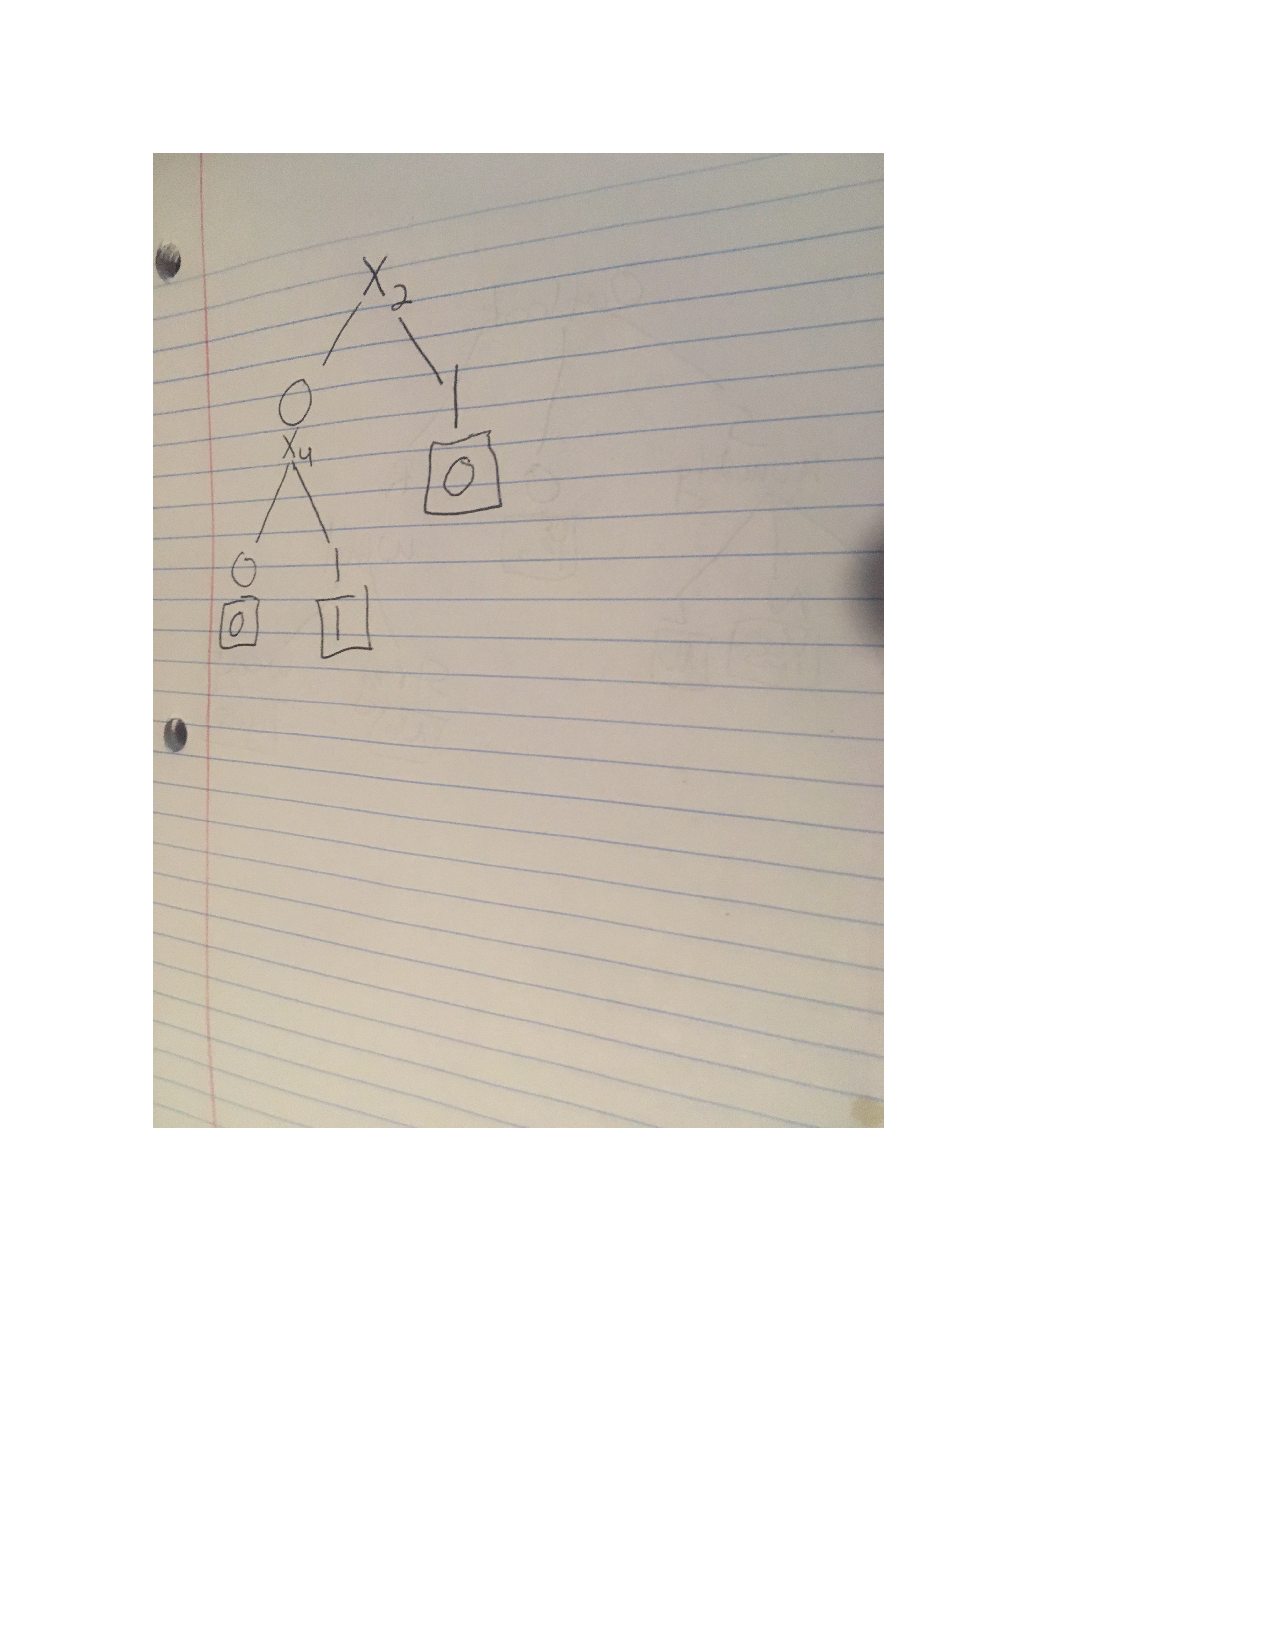
\includegraphics[scale=.65]{./p1_tree.pdf}



All of the trees for questions 2 and 3 ended up having the same structure:


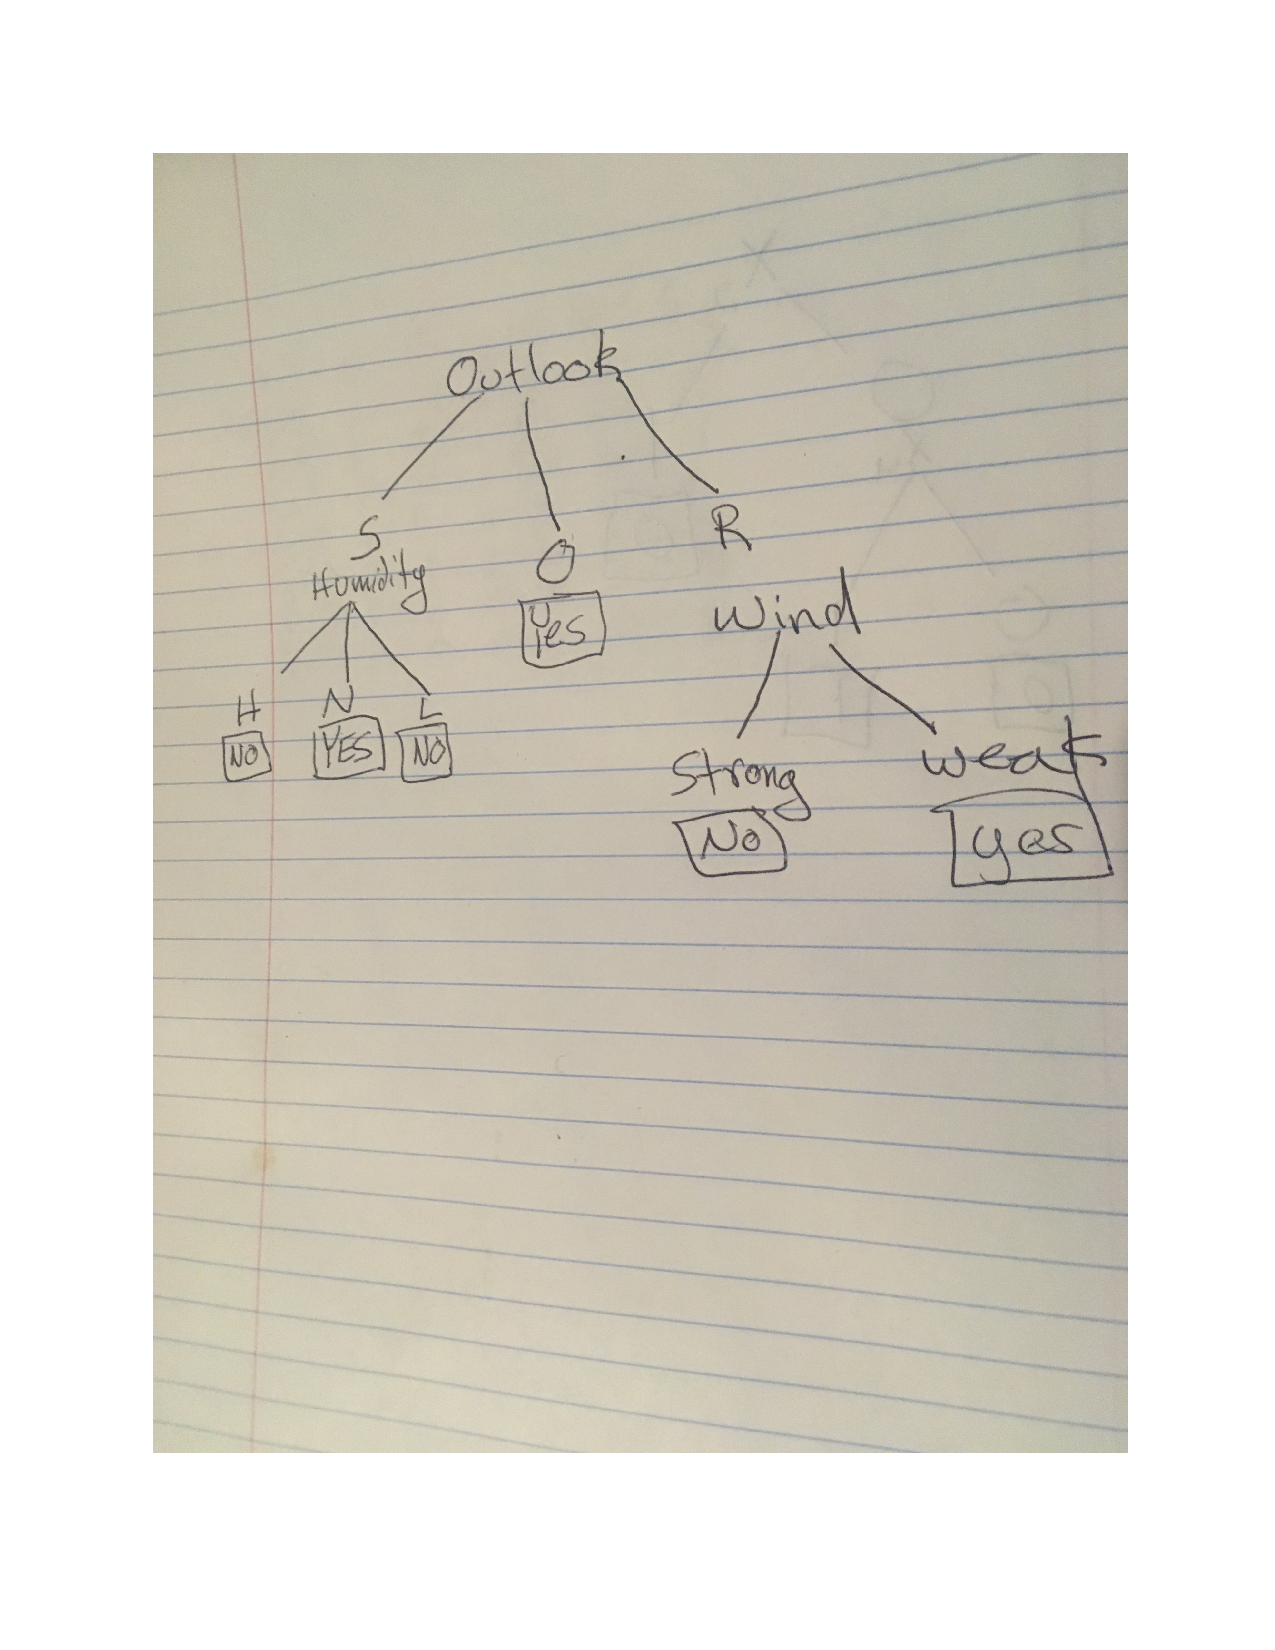
\includegraphics[scale=.6]{./tennis_tree.pdf}


\end{document}
%%% Local Variables:
%%% mode: latex
%%% TeX-master: t
%%% End:
